\subsection{PCB Schematics}
\label{sec:pcbSchematics}
Red is traces pulled on the top layer and blue are the traces on the bottom layer.
\begin{figure}[H]
    \centering
    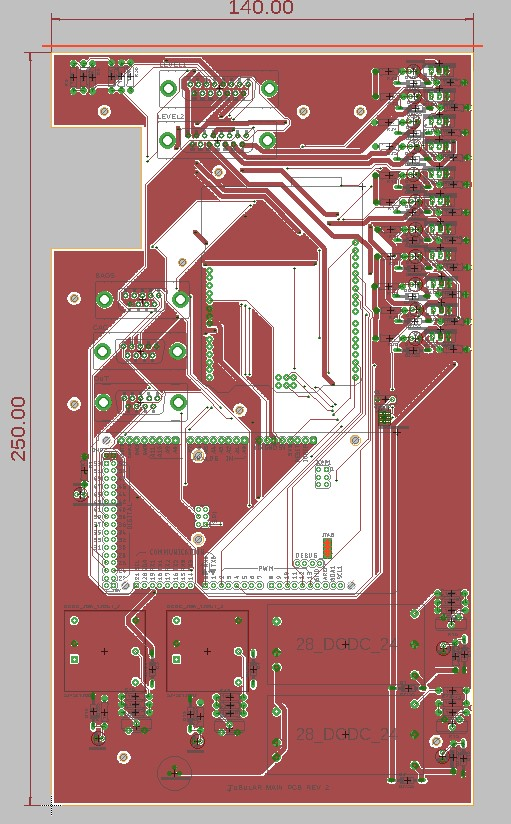
\includegraphics[width=0.75\textwidth]{appendix/img/MainPCBTop.jpg}
    \caption{Main PCB Top layer Layout in Eagle.}
    \label{fig:PCBinEagle}
\end{figure}

\begin{figure}[H]
    \centering
    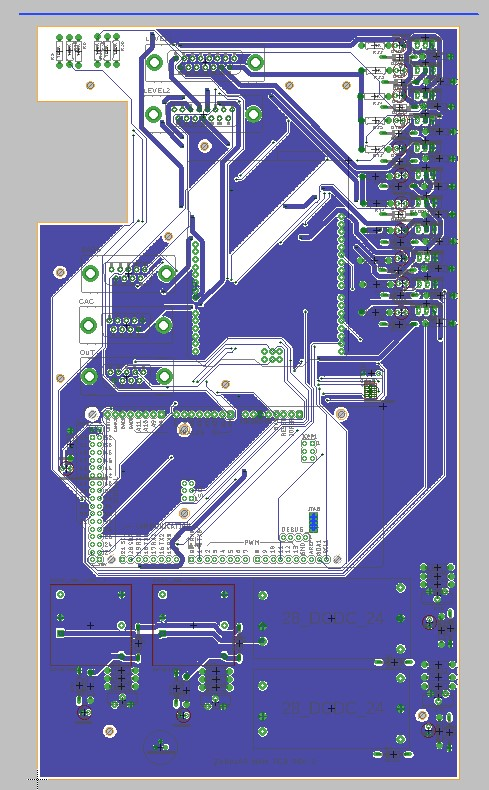
\includegraphics[width=0.75\textwidth]{appendix/img/MainPCBBot.jpg}
    \caption{Main PCB bottom layer Layout in Eagle.}
    \label{fig:PCBinEagle}
\end{figure}

\begin{figure}[H]
    \centering
    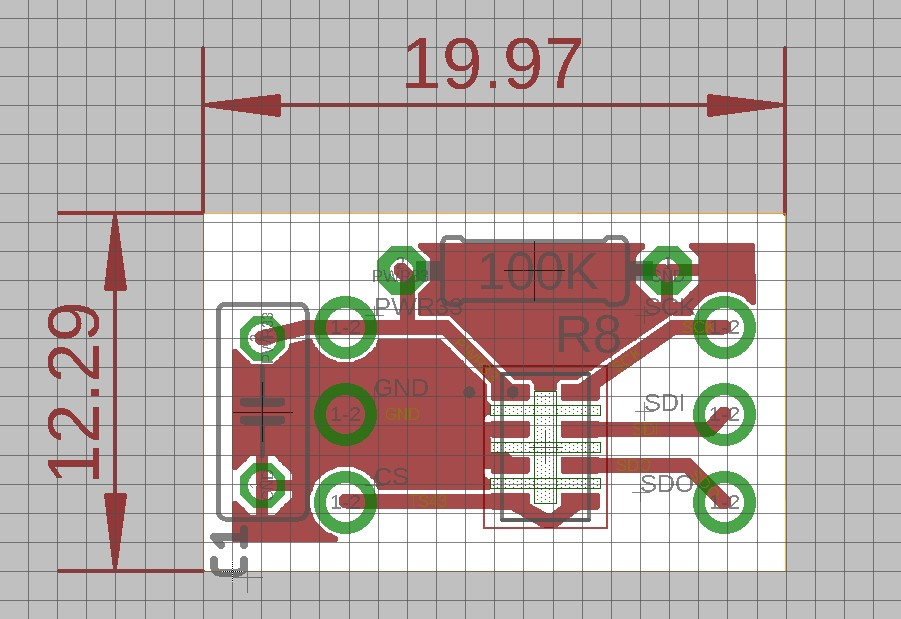
\includegraphics[width=0.75\textwidth]{appendix/img/PresPCBTop.jpg}
    \caption{Barometric pressure sensor PCB top layer Layout in Eagle.}
    \label{fig:PCBinEagle}
\end{figure}

\begin{figure}[H]
    \centering
    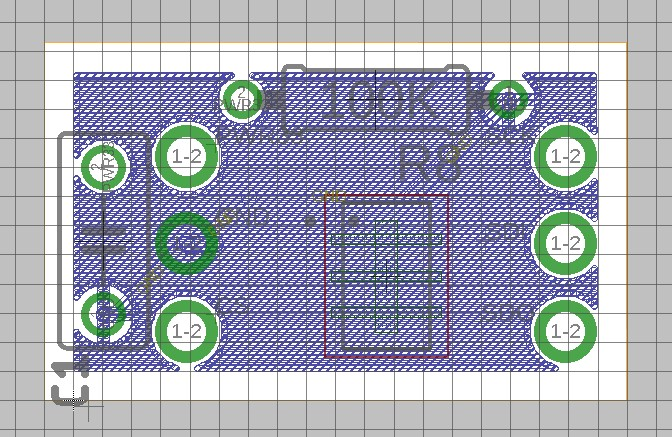
\includegraphics[width=0.75\textwidth]{appendix/img/PresPCBBot.jpg}
    \caption{Barometric pressure sensor PCB bottom layer Layout in Eagle.}
    \label{fig:PCBinEagle}
\end{figure}
